\documentclass{beamer}
\usetheme{metropolis}           % Use metropolis theme
% additional config
\usepackage[at]{easylist} % list utility
\usepackage{booktabs} % table toprule, midrule, bottomrule
\usepackage[utf8]{inputenc}
\usepackage{listings}
\usepackage{xcolor}
\usepackage{color}
\usepackage{hyperref}

\newcommand{\changeurlcolor}[1]{\hypersetup{urlcolor=#1}}  
\usepackage[absolute,overlay]{textpos}
\usepackage{graphicx}
%\usepackage{subfig}
\usepackage{bm}
\usepackage{subfigure}
\graphicspath{{figures/}}
% colors define
\definecolor{pblue}{rgb}{0.13,0.13,1}
\definecolor{pgreen}{rgb}{0,0.5,0}
\definecolor{pred}{rgb}{0.9,0,0}
\definecolor{pgrey}{rgb}{0.46,0.45,0.48}
\definecolor{RoyalBlue}{rgb}{0.254902,0.411765,0.882353}
\definecolor{lightgray}{rgb}{.9,.9,.9}
\definecolor{darkgray}{rgb}{.4,.4,.4}
\definecolor{purple}{rgb}{0.65, 0.12, 0.82}

\lstdefinelanguage{JavaScript}{
  keywords={typeof, new, true, false, catch, function, return, null, catch, switch, var, if, in, while, do, else, case, break},
  keywordstyle=\color{pred}\bfseries,
  ndkeywords={class, export, boolean, throw, implements, import, this},
  ndkeywordstyle=\color{pgrey}\bfseries,
  identifierstyle=\color{black},
  sensitive=false,
  comment=[l]{//},
  morecomment=[s]{/*}{*/},
  commentstyle=\color{purple}\ttfamily,
  stringstyle=\color{pblue}\ttfamily,
  morestring=[b]',
  morestring=[b]"
}

\lstset{
   language=JavaScript,
   backgroundcolor=\color{lightgray},
   extendedchars=true,
   basicstyle=\footnotesize\ttfamily,
   showstringspaces=false,
   showspaces=false,
   numbers=left,
   numberstyle=\footnotesize,
   numbersep=9pt,
   tabsize=2,
   breaklines=true,
   showtabs=false,
   captionpos=b
}

\title{Neural Network and TensorFlow}
\date{\today}
\author{Dapeng Hu, Qinglong Tian, Haozhe Zhang, Min Zhang}
\institute{STAT 580 Statistical Computing\\Department of Statistics\\ Iowa State University}

\setbeamertemplate{blocks}[default]

\begin{document}
\maketitle

%\begin{frame}
%	\begin{figure}
%		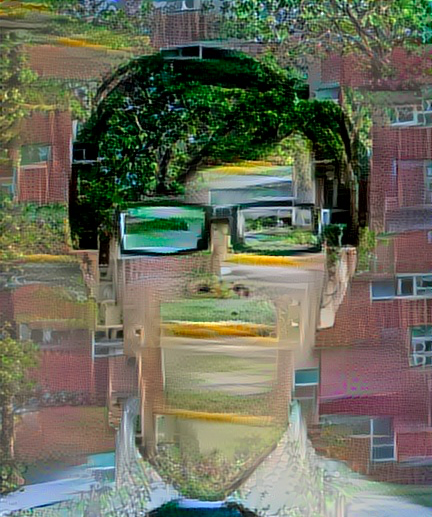
\includegraphics[width=0.59\linewidth]{style_transfer.png}
%	\end{figure}
%\end{frame}

\begin{frame}
\frametitle{Content}
\setbeamertemplate{section in toc}[sections numbered]
\tableofcontents[hideallsubsections]
\end{frame}


%\section{Why Deep Learning?}


\section{History of Neural Network}

\begin{frame}
	\frametitle{History of Neural Networks}
\begin{itemize}
	\item The 1940s: The Beginning of Neural Networks
\item The 1950s and 1960s: The First Golden Age of
Neural Networks
\item The 1970s: The Quiet Years
\item The 1980s: Renewed Enthusiasm
\end{itemize}
\end{frame}

\begin{frame}
	\frametitle{The 1940s: The Beginning of Neural Networks}
	McCulloch and Pitts, 1943
	\begin{itemize}
		\item Employed logic and mathematical notion of
		computation to explain how neural mechanism
		might realize mental functions.
		\item Commonly regarded as the inception of artificial
		neural networks.
	\end{itemize}
\end{frame}

\begin{frame}
	\frametitle{The 1940s: The Beginning of Neural Networks}
	McCulloch and Pitts, 1943
	\begin{itemize}
		\item Employed logic and mathematical notion of
		computation to explain how neural mechanism
		might realize mental functions.
		\item Commonly regarded as the inception of artificial
		neural networks.
	\end{itemize}
\end{frame}

\begin{frame}
	\frametitle{The 1940s: The Beginning of Neural Networks}
	Hebb’s Learning Rule:
	\begin{itemize}
		\item  Connectionism
		\item  A method of determining how to alter the weights between model neurons.
	\end{itemize}
	\vspace{2in}
	\begin{textblock*}{0.65\linewidth}(7cm,3.5cm) % {block width} (coords)
		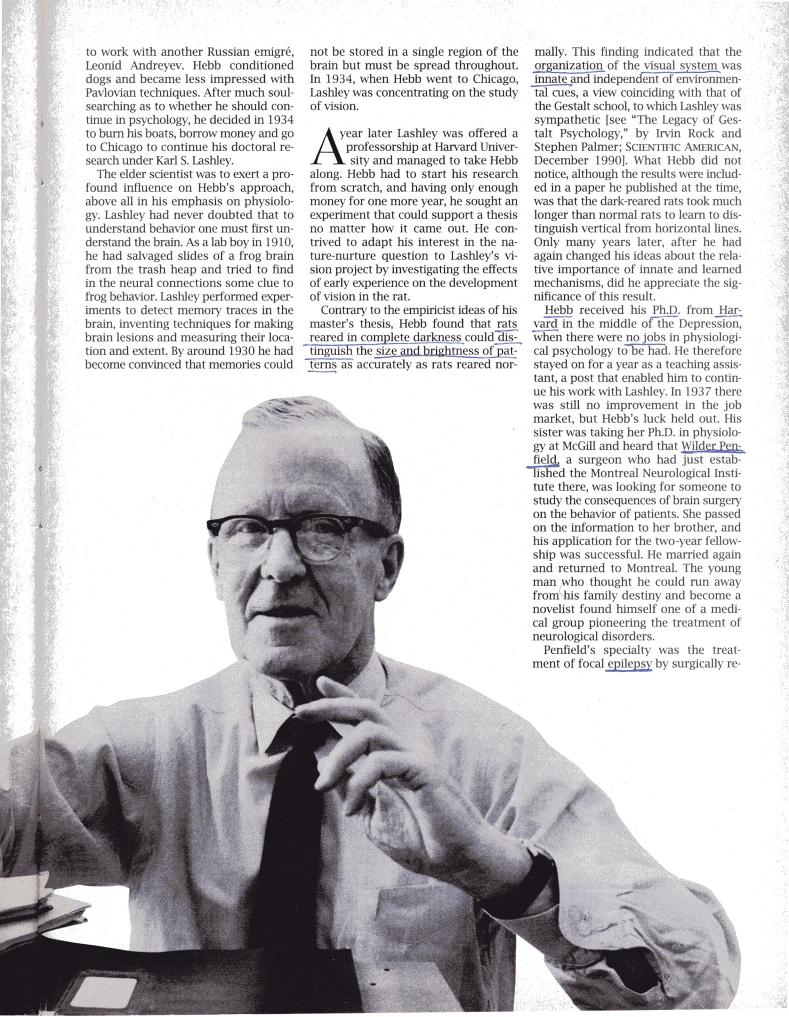
\includegraphics[width=0.65\linewidth]{image315}
	\end{textblock*}

\end{frame}


\begin{frame}
	\frametitle{The 1950s and 1960s: First Golden Age of Neural Networks}
	Perceptron (Rosenblatt’s perceptron), 1957
\begin{figure}
	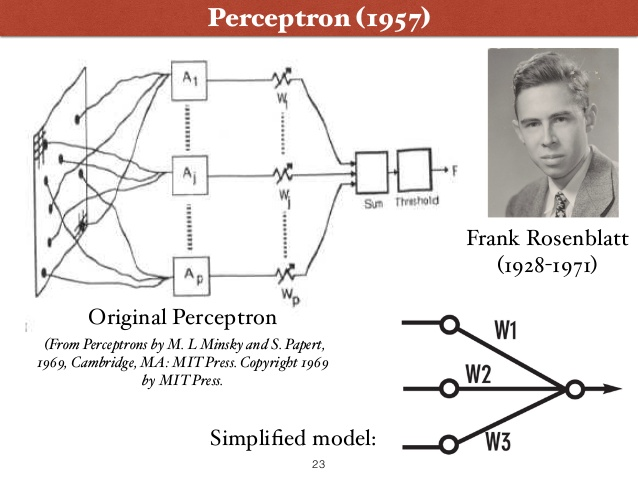
\includegraphics[width=0.75\linewidth]{perceptron-2}
\end{figure}
\end{frame}

\begin{frame}
	\frametitle{The 1970s: The Quiet Years}
	Marvin Minsky
	\begin{itemize}
		\item  “Perceptron”, 1969.
		\item “Fatal flaw” of the perceptron; inability to solve
		non-linear problems.
	\end{itemize}
\end{frame}

\begin{frame}
	\frametitle{The 1970s: The Quiet Years}
	Kunihiko Fukishima
	\begin{itemize}
		\item  Neocognitron
	\end{itemize}
	Teuvo Kohonen
	\begin{itemize}
		\item  Self-Organizing Map (SOM) algorithm
	\end{itemize}
\end{frame}

\begin{frame}
	\frametitle{The 1980s: Renewed Enthusiasm}
	John Hopfield
	\begin{itemize}
		\item  Hopfield Neural Network, 1982
	\end{itemize}
	Geoffrey Hinton, etc.
	\begin{itemize}
		\item  Blotzmann Machine
		\item Back-propagation (BP) algorithm
	\end{itemize}
\end{frame}

\section{Neural Network}
\begin{frame}
	\frametitle{A Neuron Model}
	\begin{figure}
		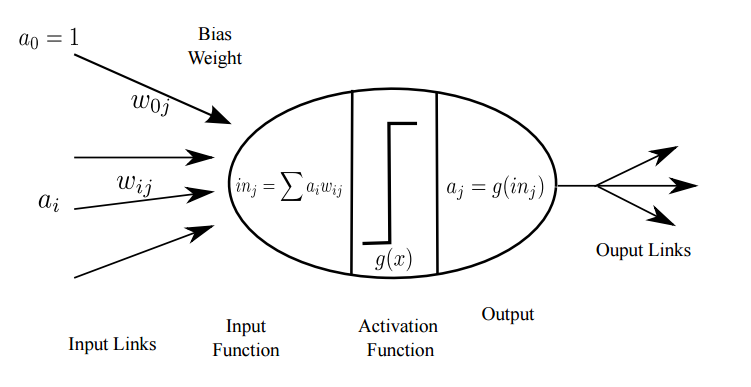
\includegraphics[width=0.95\linewidth]{neuron_model}
	\end{figure}
\end{frame}

\begin{frame}
	\frametitle{A Neuron Model}
\begin{itemize}
	\item The weights of the neuron are the parameters of the model.
	\item The input is computed as a weighted sum of the inputs.
	\item The activation function determines the output and can be different functions.
	\item The output is obtained by applying the activation function to the input.
	\item \href{https://appliedgo.net/perceptron/}{ \textcolor{pblue}{How does the neuron work?}}
\end{itemize}
\end{frame}

\begin{frame}
	\frametitle{A Neuron Model}
	\begin{figure}
		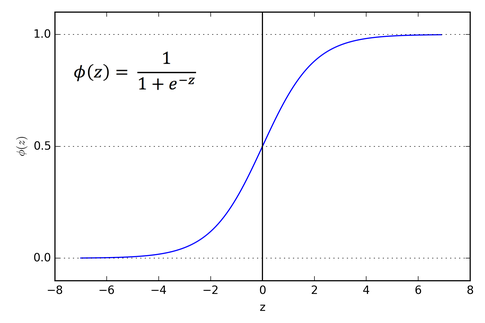
\includegraphics[width=0.8\linewidth]{sigmoid.png}
	\end{figure}
\end{frame}

\begin{frame}
	\frametitle{Single-layer Neural Network}
	\begin{figure}
		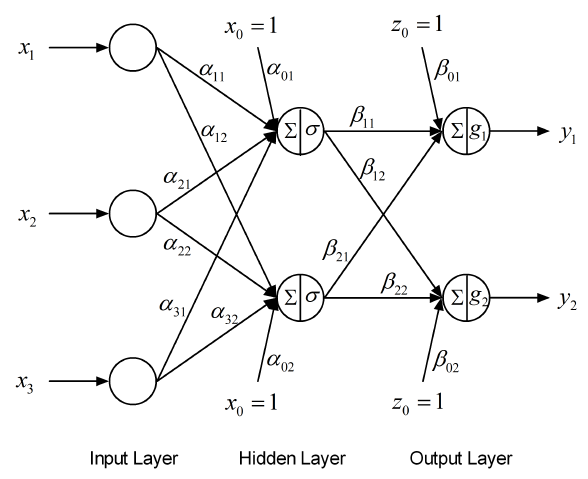
\includegraphics[width=0.8\linewidth]{singlelayer_network1.png}
	\end{figure}
\end{frame}

\begin{frame}
	\frametitle{Multiple-layer Neural Network}
	\begin{figure}
		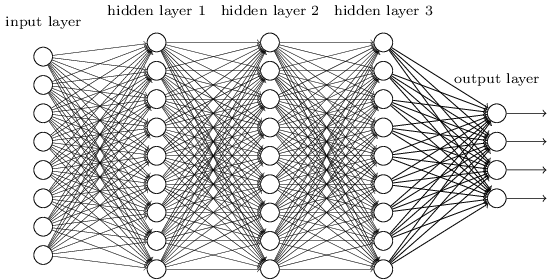
\includegraphics[width=0.8\linewidth]{multilayer_network.png}
	\end{figure}
\end{frame}

\begin{frame}
	\frametitle{Delta Learning Rule}
\begin{itemize}
	\item Based on gradient descent algorithm.
	\item Only applicable for continuous activation function.
	\item The learning signal r is called delta and defined as:
	\begin{equation*}
	r = \{d_{j} - f(\bm{W}_{j}^{T}\bm{X})\}f'(\bm{W}_{j}^{T}\bm{X}) \approx (d_{j}-o_{j})f'(\text{net}_{j})
	\end{equation*}
	\item The weights will be adjusted as:
	\begin{equation*}
	\Delta \bm{W}_{j} = \eta(d_{j} - o_{j})f'(\text{net}_{j})\bm{X}
	\end{equation*}
	
\end{itemize}
\end{frame}

\begin{frame}
	\frametitle{Backpropagation Algorithm}
	\begin{itemize}
		\item BP algorithm is a process of training a neural network
		\item Based on delta learning rule
	\end{itemize}
	\begin{figure}
		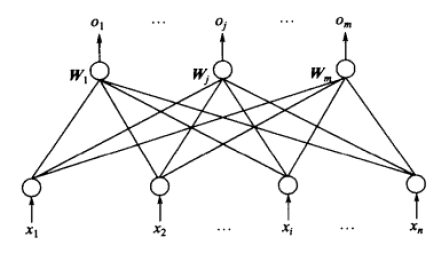
\includegraphics[width=0.8\linewidth]{singlelayer_network.png}
	\end{figure}
\end{frame}

\begin{frame}
	\frametitle{Backpropagation Algorithm}
\begin{itemize}
	\item For the output layer
	\begin{equation*}
	\Delta \omega_{jk}^{h+1} = \eta\delta_{k}^{h+1}y_{j}^{h}=\eta(d_{k}-o_{k})o_{k}(1-o_{k})y_{j}^{h},
	\end{equation*}
	where $j=0,\ldots, m_{h}$, $k=1,\ldots,\ell$.
	\item For the $h$th hidden layer
		\begin{equation*}
		\Delta \omega_{ij}^{h} =\eta \delta_{j}^{h}y_{i}^{h-1} = \eta\left(\sum_{k=1}^{l}\delta_{k}^{o}\omega_{jk}^{h+1}\right)y_{j}^{h}(1-y_{j}^{h})y_{i}^{h-1}.
		\end{equation*}
			where $i=0,\ldots, m_{h-1}$, $j=1,\ldots,m_{h}$.
	\item The first hidden layer
		\begin{equation*}
		\Delta \omega_{pq}^{1} =\eta\delta_{q}^{1}x_{p}= \eta\left(\sum_{r=1}^{m_{2}}\delta_{r}^{2}\omega_{qr}^{2}\right)y_{q}^{1}(1-y_{q}^{1})x_{p}.
		\end{equation*}
			where $p=0,\ldots, n$, $k=1,\ldots,m_{1}$.
\end{itemize}
\end{frame}

\begin{frame}
	\frametitle{Backpropagation Algorithm}
	The flow of signal in BP algorithm:
	\begin{figure}
		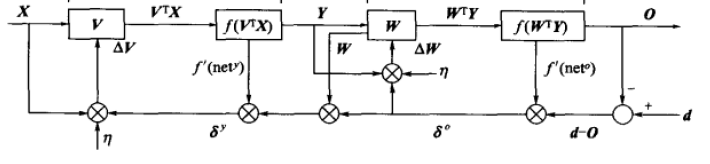
\includegraphics[width=\linewidth]{bp_flow.png}
	\end{figure}
\end{frame}

\begin{frame}
	\frametitle{More Hidden Layers?}
	\begin{itemize}
		\item The signal is getting weaker
		\item Non-convex problem
		\item Slow Convergence
		\item Weakness of Gradient Descent: Local Optima
	\end{itemize}
\end{frame}

\begin{frame}
	\frametitle{Breakthrough}
	{\small Hinton, G. E., \& Salakhutdinov, R. R. (2006). Reducing the dimensionality of data with neural networks. Science, 313(5786), 504-507.}
	\begin{figure}
		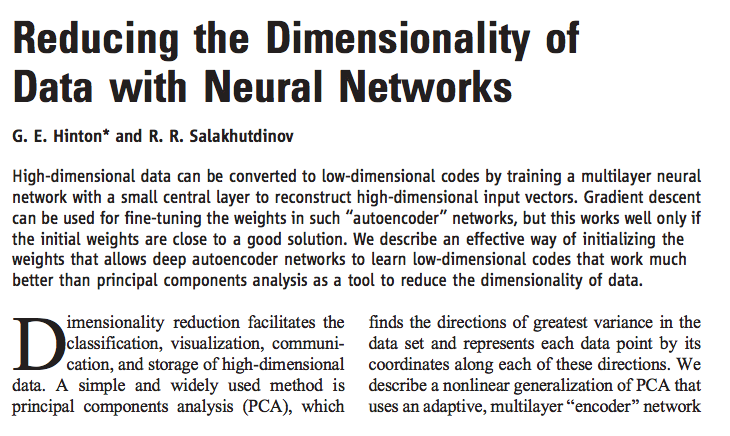
\includegraphics[width=0.95\linewidth]{breakthrough}
	\end{figure}
\end{frame}

\section{Convolutional Neural Network}
\begin{frame}
	\frametitle{CNN}
	\begin{figure}
		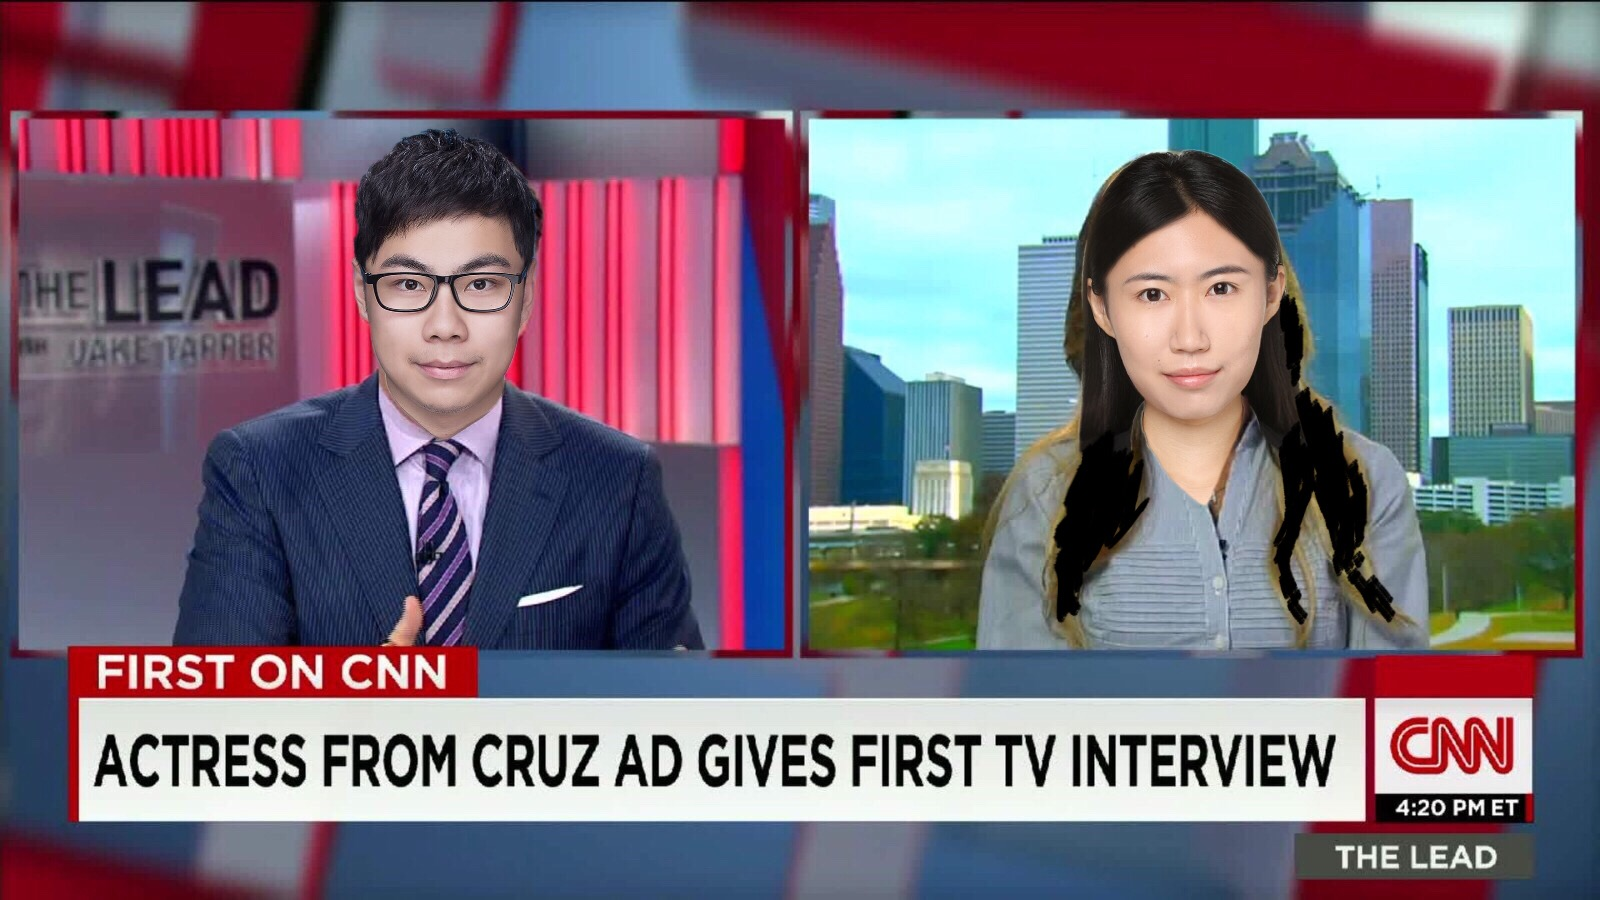
\includegraphics[width=\linewidth]{cnn_tv_dapeng}
	\end{figure}
\end{frame}

\begin{frame}
\frametitle{Why CNN?}
\begin{itemize}
	\item Fully connected neural network can bring us too many parameters.
	\item Some patterns are much smaller than the whole image.
\end{itemize}

\begin{figure}
	\hfill
\subfigure{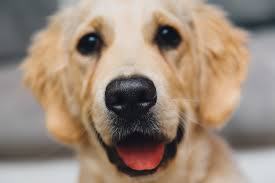
\includegraphics[width=.65\linewidth]{dog1.jpg}}
\hfill
\subfigure{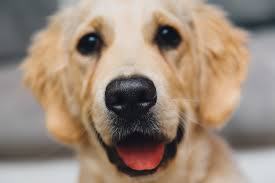
\includegraphics[width=.2\linewidth]{dog2}}
\hfill
\end{figure}

\end{frame}


\begin{frame}
	\frametitle{Why CNN?}
The same pattern appears in different regions.
	
	\begin{figure}
		\hfill
		\subfigure{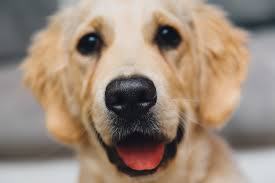
\includegraphics[width=.49\linewidth]{dog1.jpg}}
		\hfill
		\subfigure{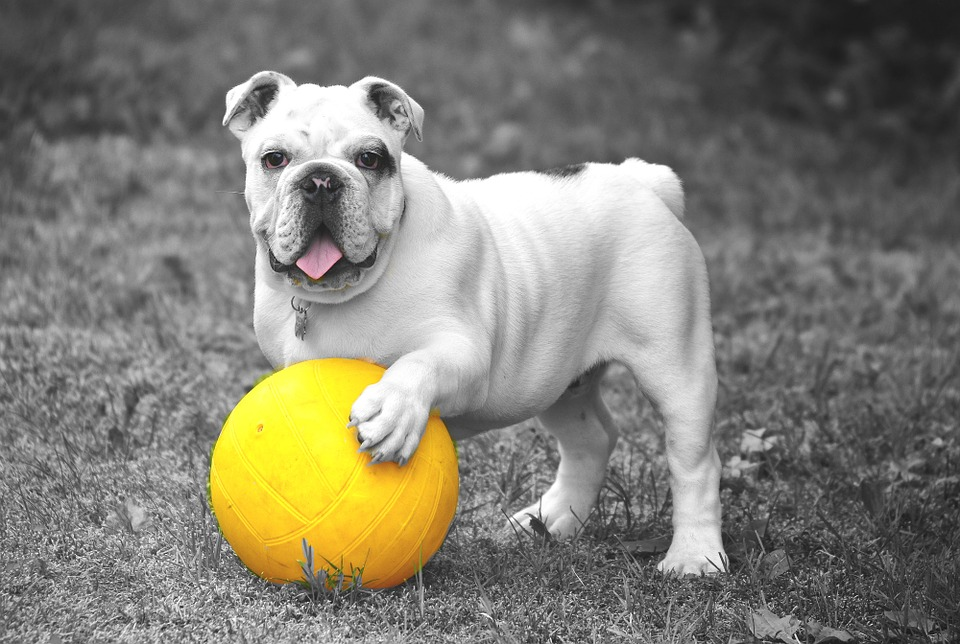
\includegraphics[width=.485\linewidth]{dog3}}
		\hfill
	\end{figure}
	
\end{frame}

\begin{frame}
	\frametitle{Why CNN?}
	Subsampling the pixels will not change the object.
	
	\begin{figure}
		\hfill
		\subfigure{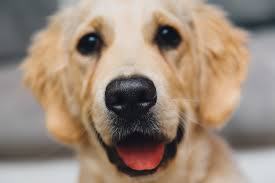
\includegraphics[width=.6\linewidth]{dog1.jpg}}
		\hfill
		\subfigure{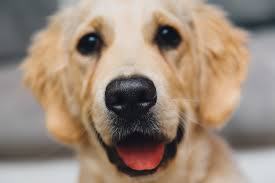
\includegraphics[width=.3\linewidth]{dog1.jpg}}
		\hfill
	\end{figure}
	
\end{frame}

\begin{frame}
	\frametitle{Whole Structure}
	\begin{figure}
	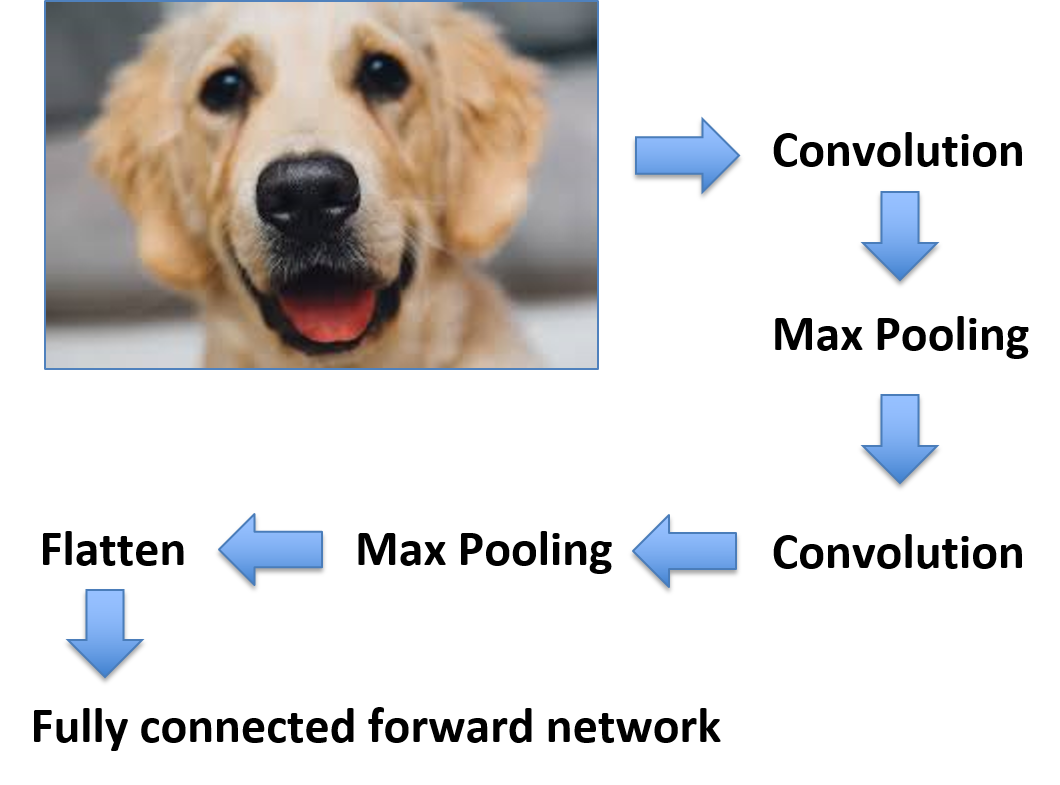
\includegraphics[width=0.8\linewidth]{Picture1}
	\end{figure}
\end{frame}

\begin{frame}
	\frametitle{How convolution works?}
	\begin{figure}
	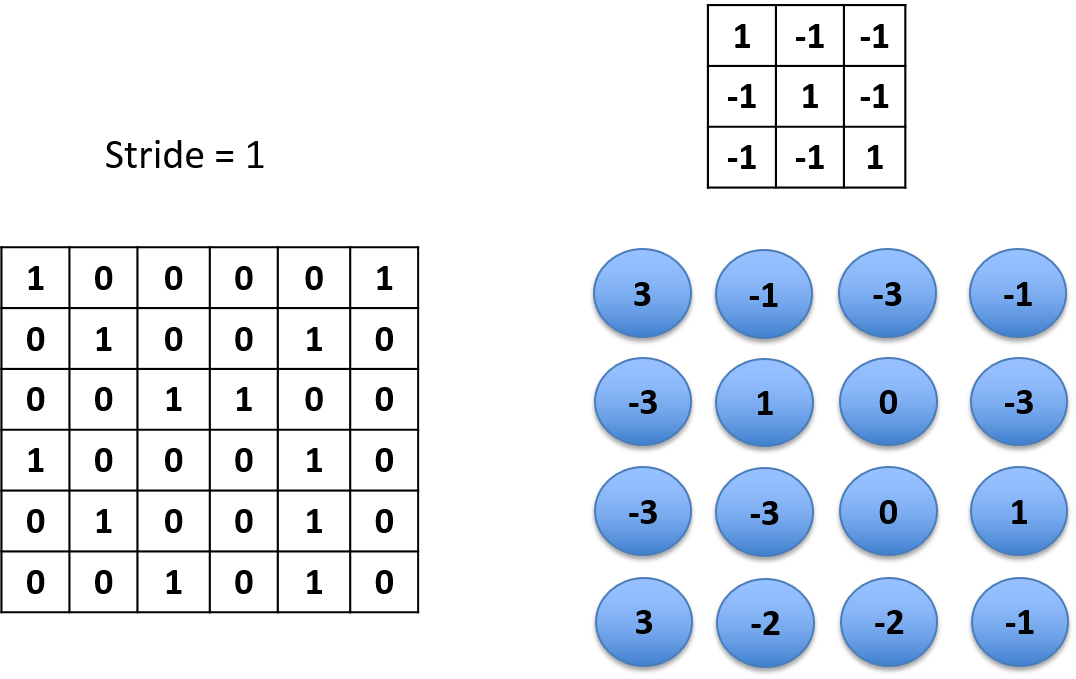
\includegraphics[width=0.8\linewidth]{Picture2}
	\end{figure}
\end{frame}

\begin{frame}
	\frametitle{How convolution works?}
	\begin{figure}
	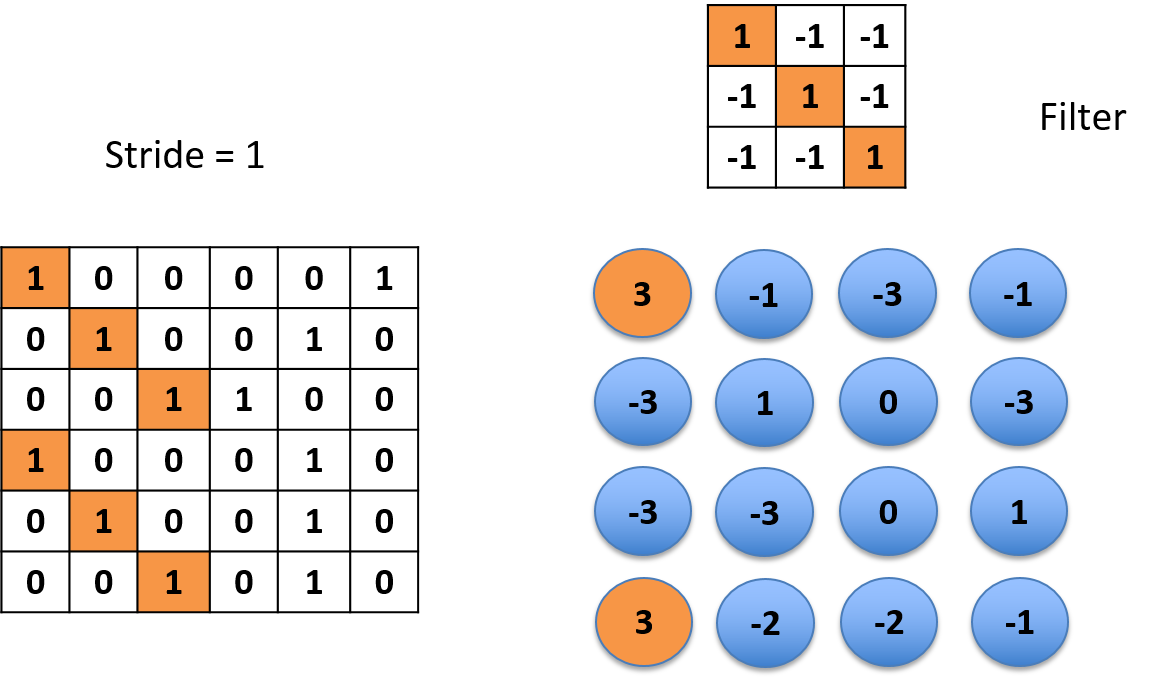
\includegraphics[width=0.8\linewidth]{Picture3}
	\end{figure}
\end{frame}

\begin{frame}
	\frametitle{How convolution works?}
	\begin{figure}
	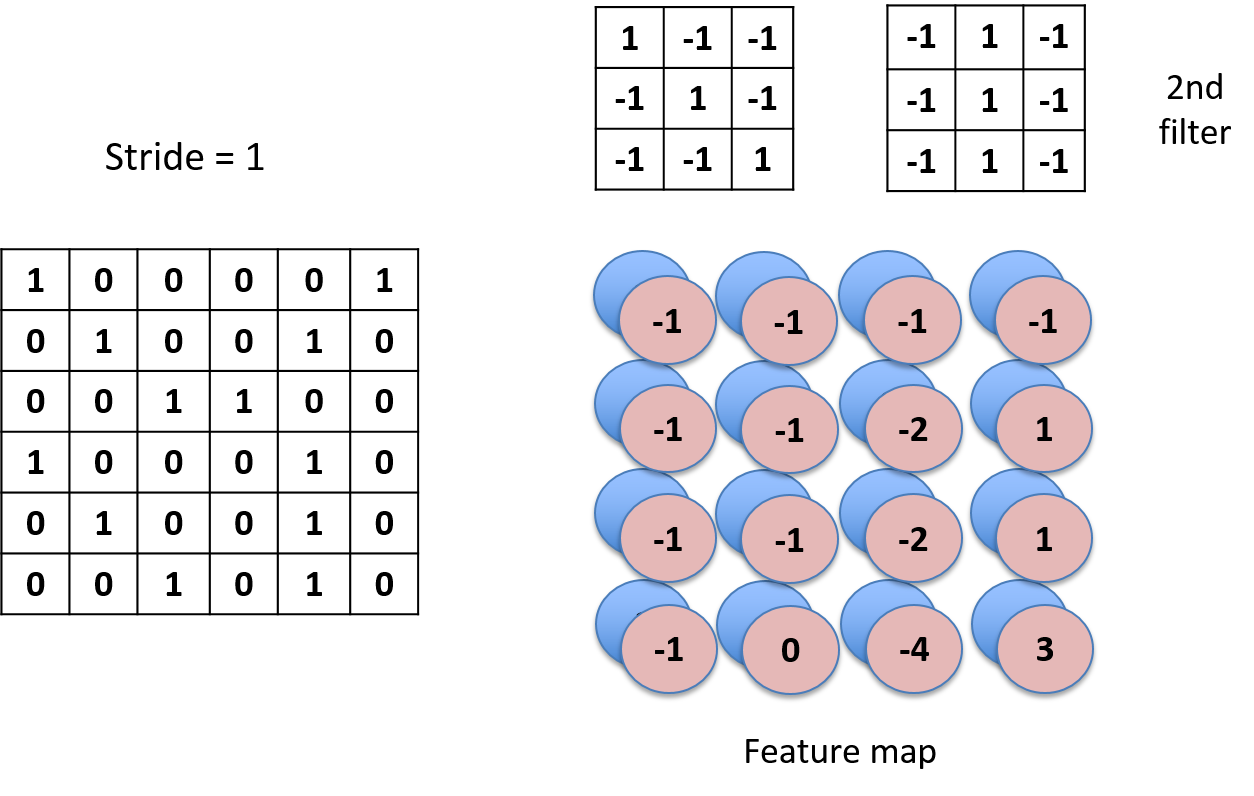
\includegraphics[width=0.8\linewidth]{Picture4}
	\end{figure}
\end{frame}

\begin{frame}
	\frametitle{Connection between CNN and Neural Network}
	\begin{figure}
		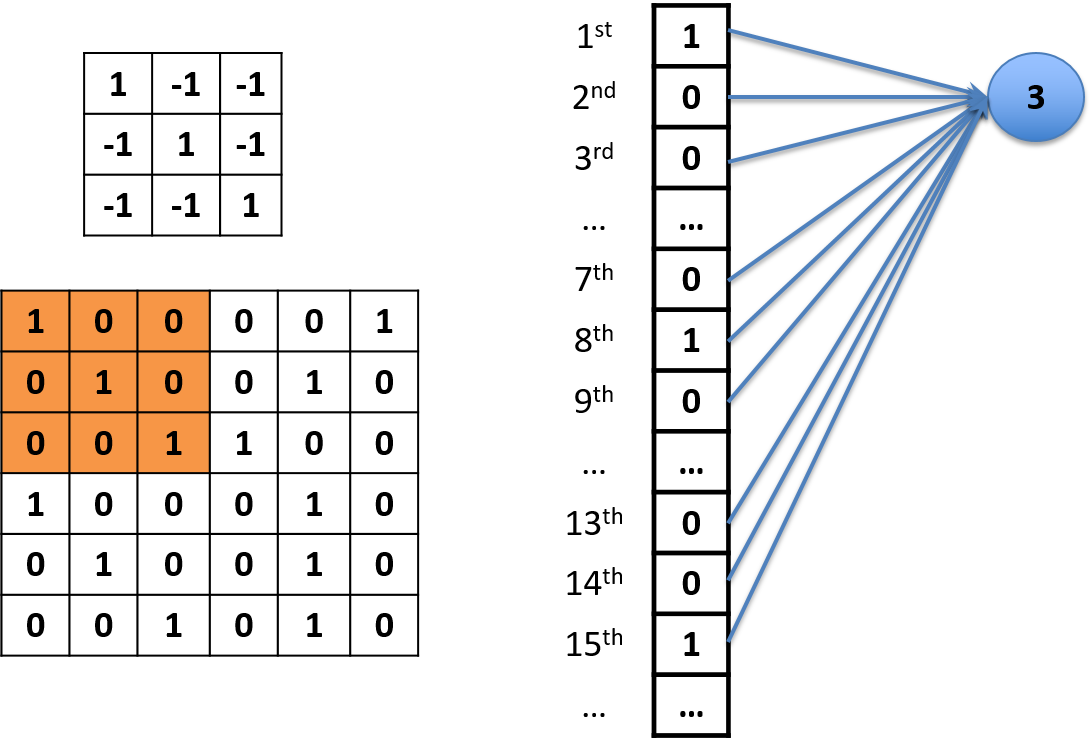
\includegraphics[width=0.8\linewidth]{Picture5}
	\end{figure}
\end{frame}

\begin{frame}
	\frametitle{Connection between CNN and Neural Network}
	\begin{figure}
	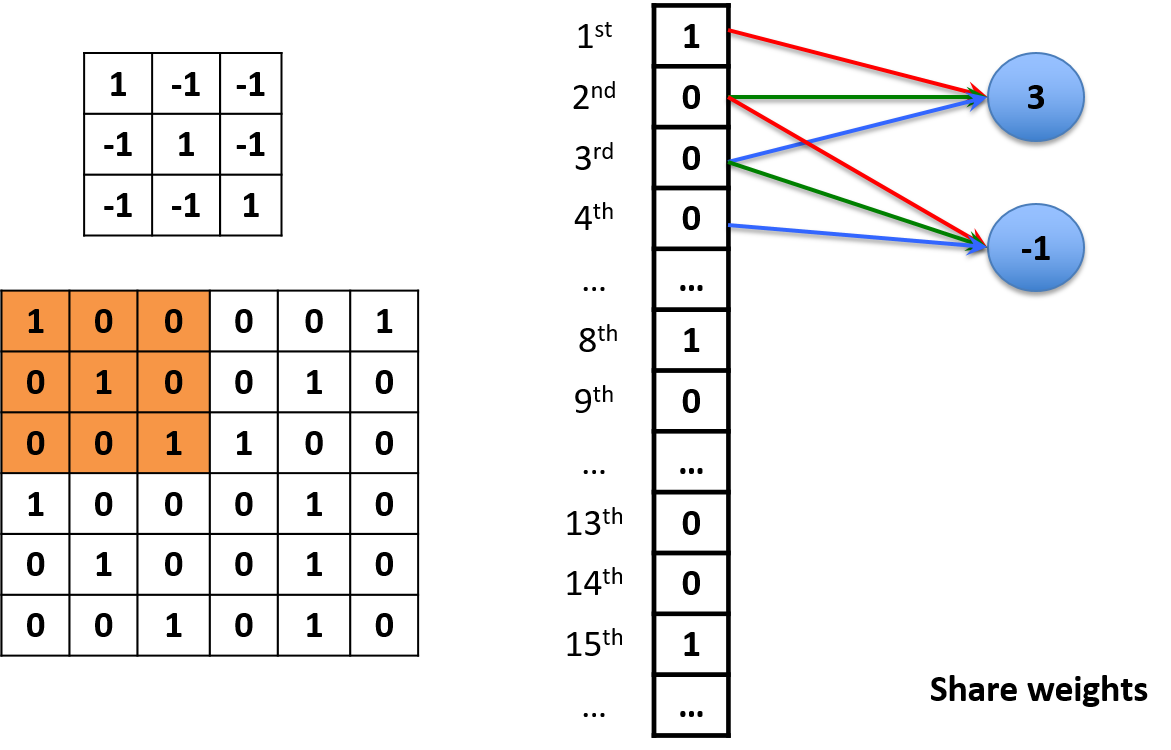
\includegraphics[width=0.8\linewidth]{Picture6}
	\end{figure}
\end{frame}

\begin{frame}
	\frametitle{Max pooling}
	\begin{figure}
		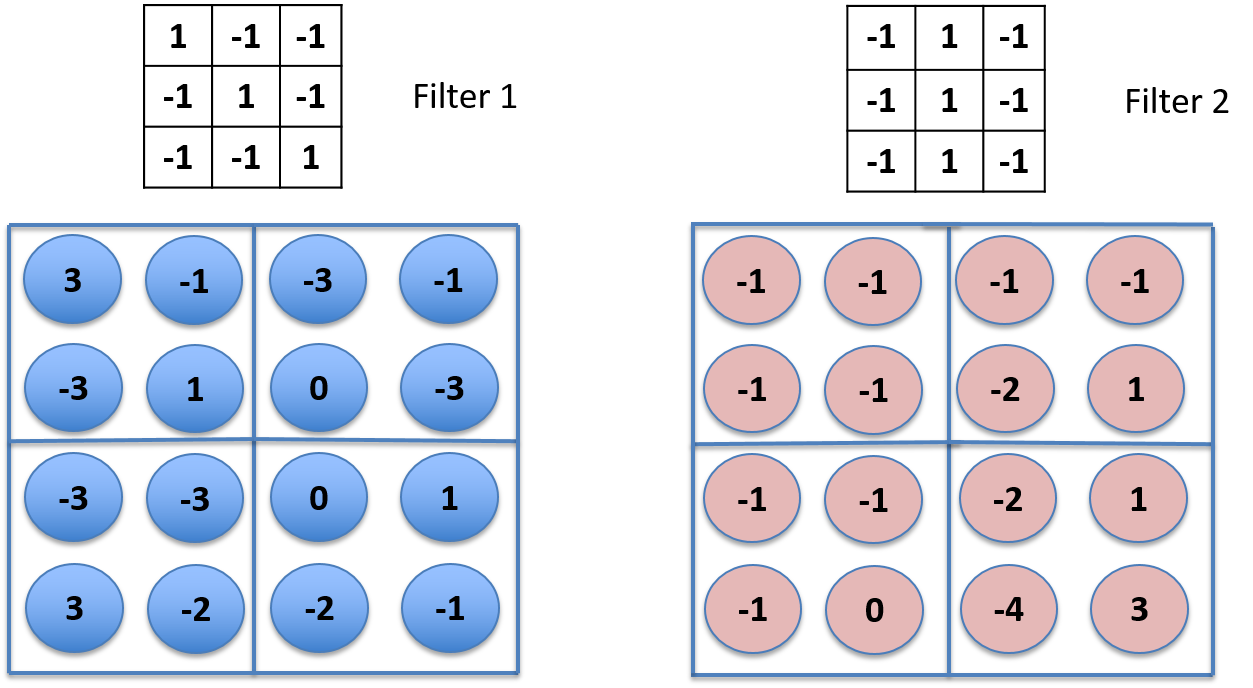
\includegraphics[width=0.8\linewidth]{Picture7}
	\end{figure}
\end{frame}

\begin{frame}
	\frametitle{Max pooling}
	\begin{figure}
	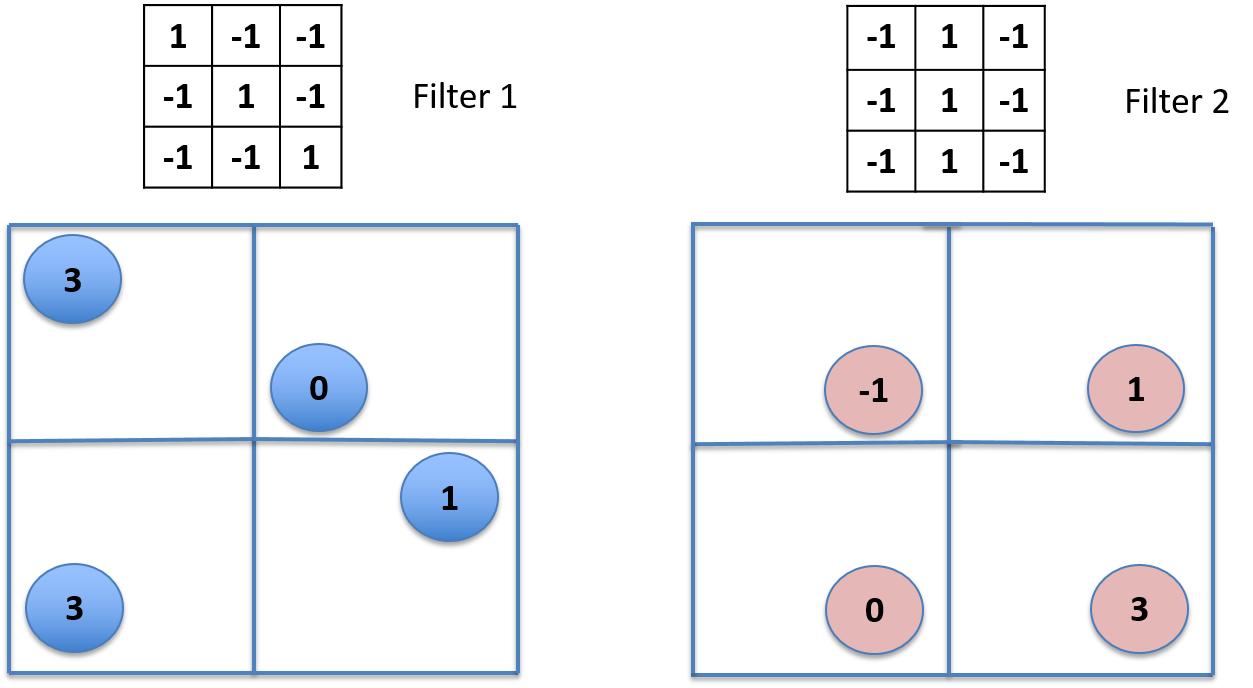
\includegraphics[width=0.8\linewidth]{Picture8}
	\end{figure}
\end{frame}

\begin{frame}
%	\frametitle{After convolution and max pooling}
	\begin{figure}
	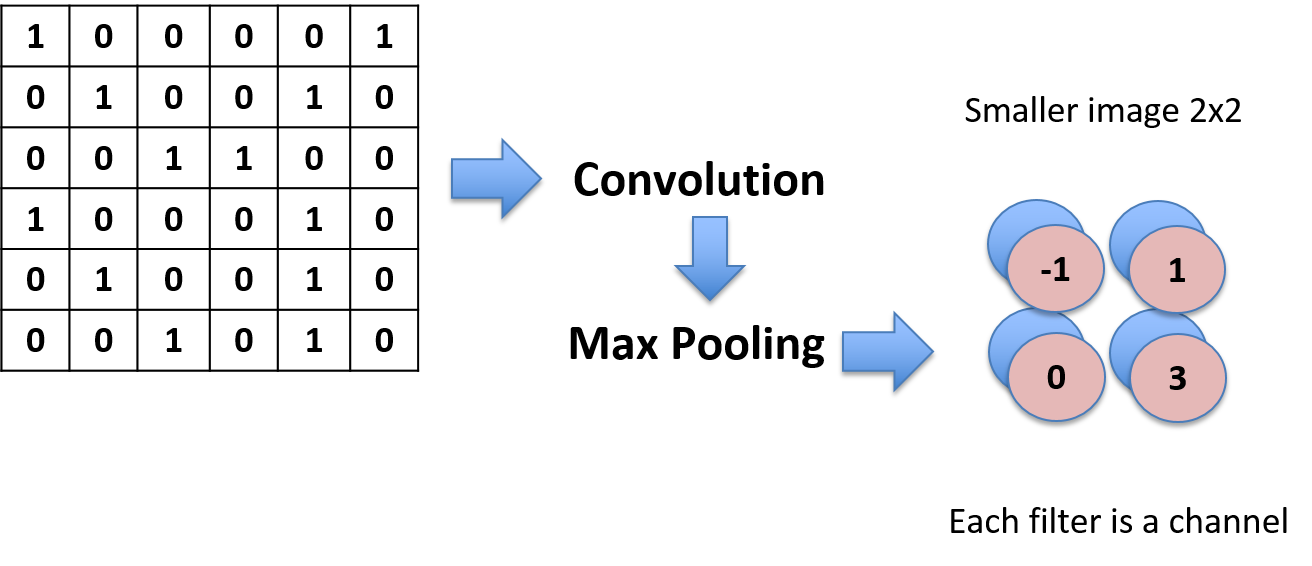
\includegraphics[width=\linewidth]{Picture9}
	\end{figure}
\end{frame}

\begin{frame}
	\frametitle{Flatten}
	\begin{figure}
	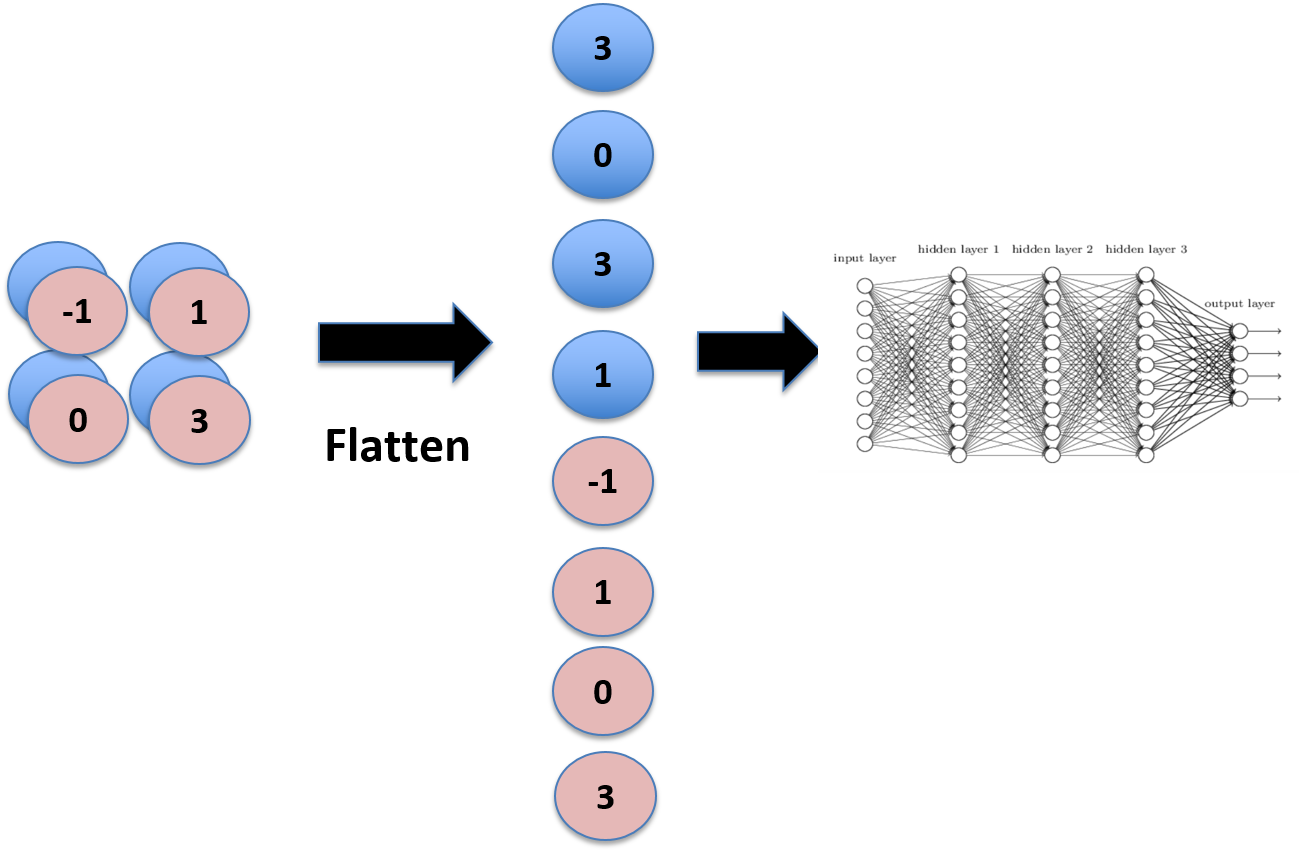
\includegraphics[width=\linewidth]{Picture10}
	\end{figure}
\end{frame}



\begin{frame}
	\frametitle{Example of CNN: MNIST}
	The MNIST dataset contains images of handwritten digits like below. Each image is 28 pixels by 28 pixels. It also includes labels for each image, telling us which digit it is. Next, we are going to train a model to look at images and predict which digits they are.
	
	\href{https://www.youtube.com/watch?v=FwFduRA_L6Q}{ \textit{\textcolor{pblue}{First Convolutional Network Demo from 1993}}}
	
	\begin{figure}
		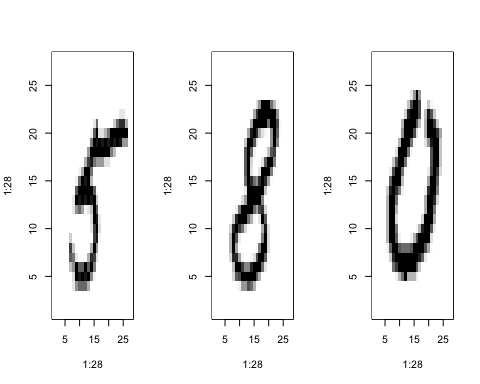
\includegraphics[width=0.9\linewidth, height=0.4\linewidth]{MNIST1}
	\end{figure}
	
\end{frame}

\section{TensorFlow}
\begin{frame}
	\frametitle{TensorFlow}
	
\vspace{0.5in}
About TensorFlow:
\begin{itemize}
	\item Tensorflow is an open source software library for numerical computation using data flow graphs. Nodes in the graph represent mathematical operations, which the graph edges represent the multidimensional data arrays (tensors) communicated between them. 
	\item It allows you to deploy computation to one or more CPUs or GPUs in d desktop, server, or mobile device with a single API. The Tensorflow package provide access to the complete Tensorflow API from within R. 
\end{itemize}
%	\begin{figure}
%		
\includegraphics[width=0.55\linewidth]{tensorflow_logo}
%	\end{figure}
	\begin{textblock*}{5cm}(10cm,1cm) % {block width} (coords)
		
\includegraphics[width=2.5cm]{tensorflow_logo}
	\end{textblock*}
\end{frame}

\begin{frame}
	\frametitle{MNIST}
mnist\$train\$image is a tensor (an n-dimensional array) with shape ($55000$L, $784$L). 
	\begin{figure}
		
\includegraphics[width=0.8\linewidth]{MNIST2}
	\end{figure}
\end{frame}


\begin{frame}
	\frametitle{MNIST}
	The label is ``one-hot vectors". \\
	For example, $3$ would be [$0,0,0,1,0,0,0,0,0,0$]\.\
	mnist\$train\$labels is a tensor with shape ($55000$L, $10$L). 
	\begin{figure}
		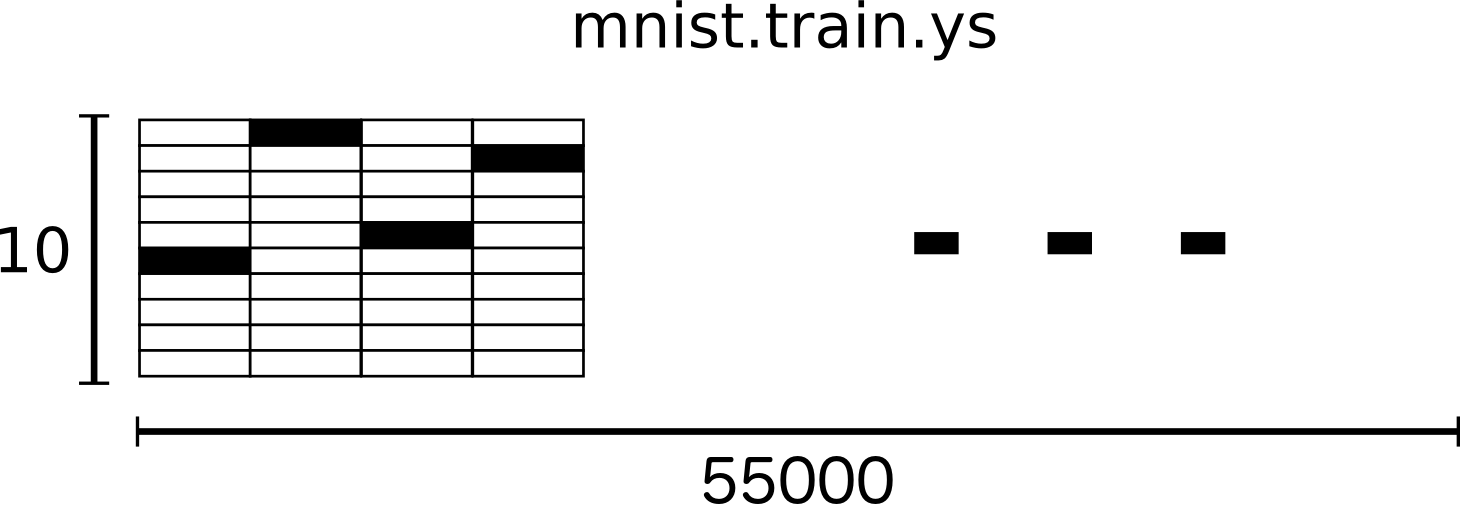
\includegraphics[width=0.8\linewidth]{MNIST3}
	\end{figure}
\end{frame}

\begin{frame}
	\frametitle{MNIST}
	Why do we have 2 layers, not more?\\
	Vanishing Gradient Problem $\longrightarrow$ Deeper does not usually imply better.
	\begin{figure}
		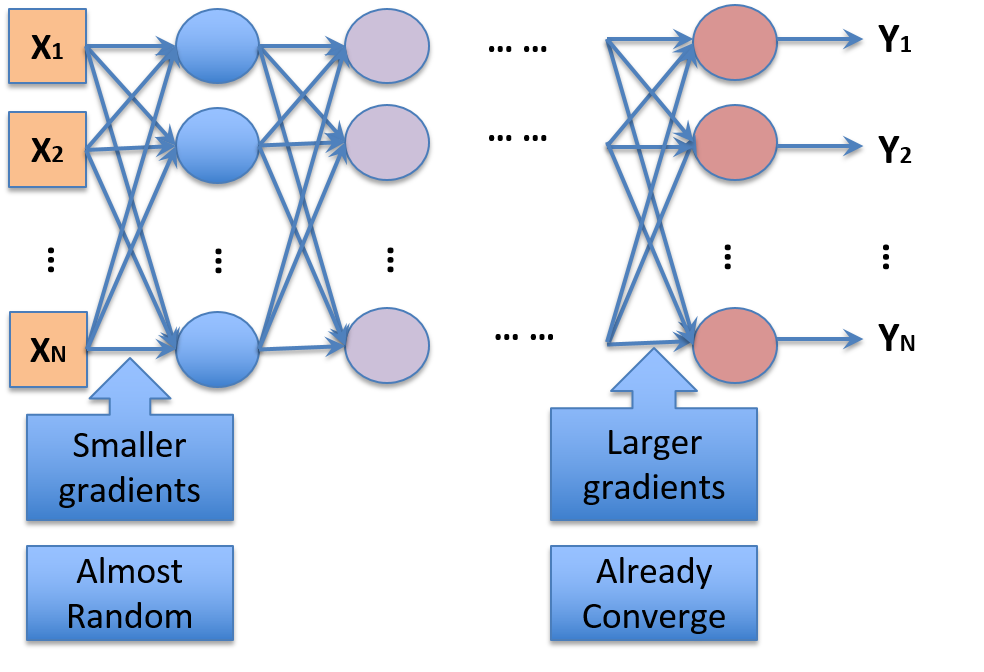
\includegraphics[width=0.8\linewidth]{Picture14}
	\end{figure}
\end{frame}

\begin{frame}
	\frametitle{MNIST}
Activation function: Rectified Linear Unit (ReLU)\\
Reason:
\begin{itemize}
		\item Infinite sigmoid with different biases
		\item Able to handle vanishing gradient problem
	\item Fast to compute
	\item Biological reason
\end{itemize}
\vspace{1.5in}

\begin{textblock*}{5cm}(7cm,4cm) % {block width} (coords)
	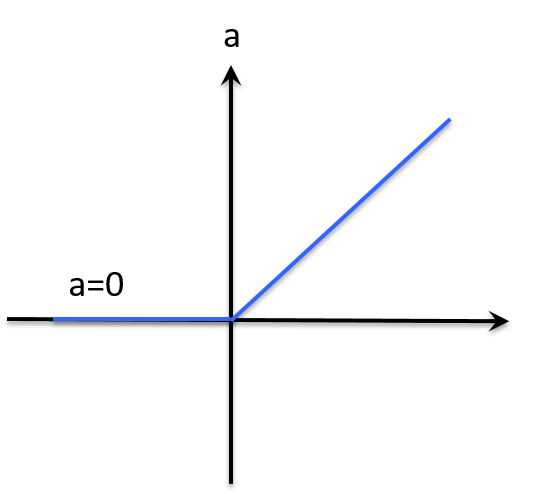
\includegraphics[width=5cm]{Picture15}
\end{textblock*}
\end{frame}

\begin{frame}
	\frametitle{MNIST}
Dropout: when you do training, each time before updating the parameters, each neuron has p\% to dropout.
	\begin{figure}
		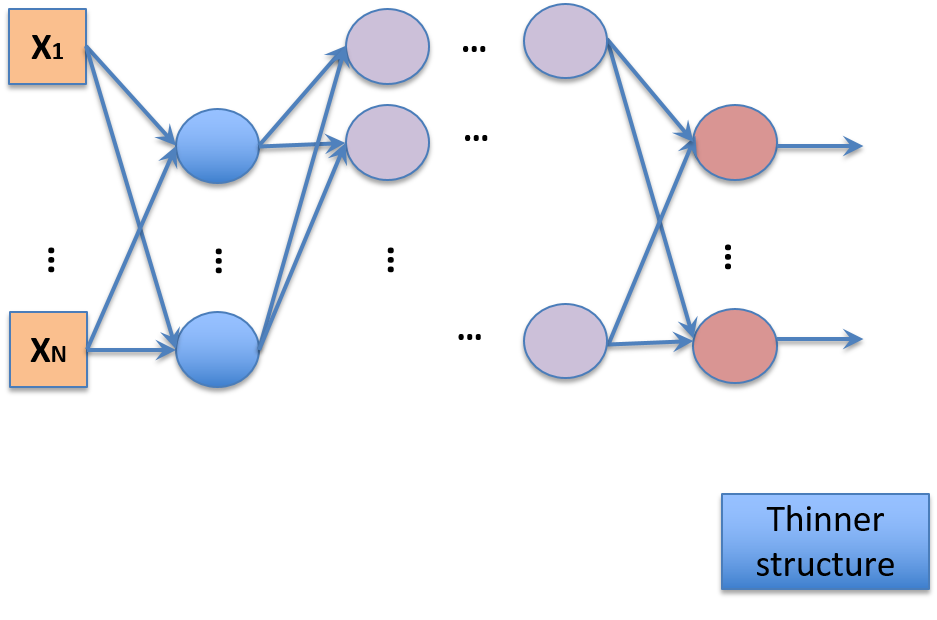
\includegraphics[width=0.8\linewidth]{Picture16}
	\end{figure}
\end{frame}


\begin{frame}
	\frametitle{CNN Visualization: Example of MNIST}
\begin{center}
\href{http://scs.ryerson.ca/~aharley/vis/conv/}{ \textit{\textcolor{pblue}{3D convolutional network visualization}}}
\end{center}
	\begin{figure}
		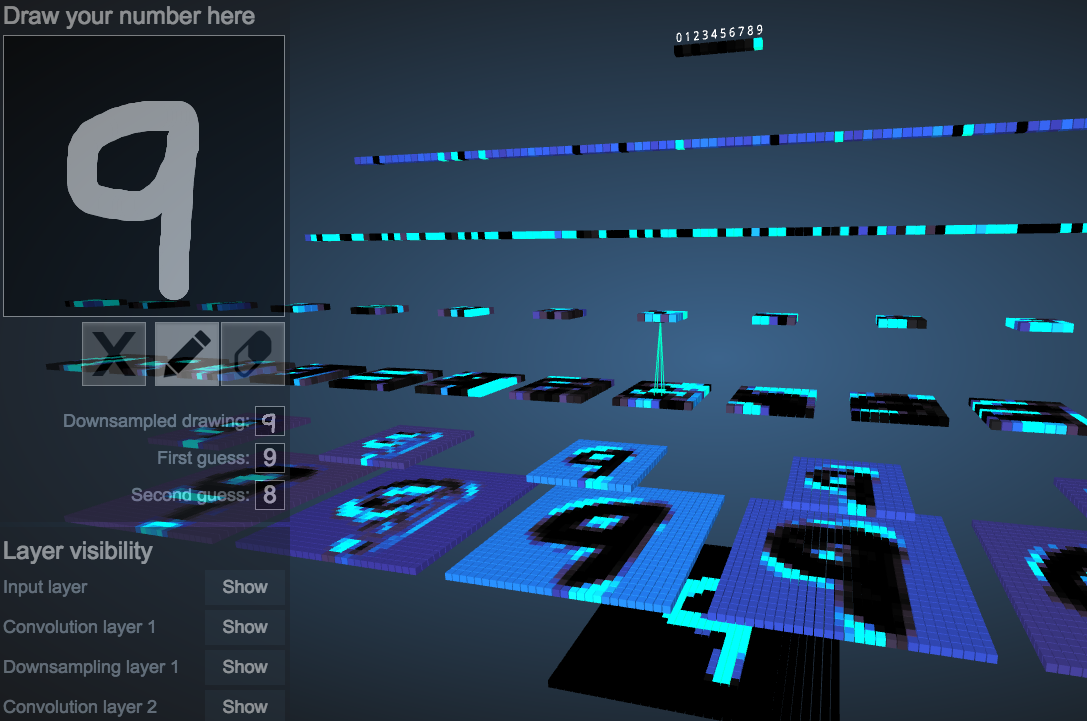
\includegraphics[width=0.95\linewidth]{cnn_visualization}
	\end{figure}
\end{frame}

\begin{frame}
	\frametitle{Style Transfer}
\begin{center}
Style Transfer, A.K.A. Deep Style
\end{center}
	\begin{figure}
		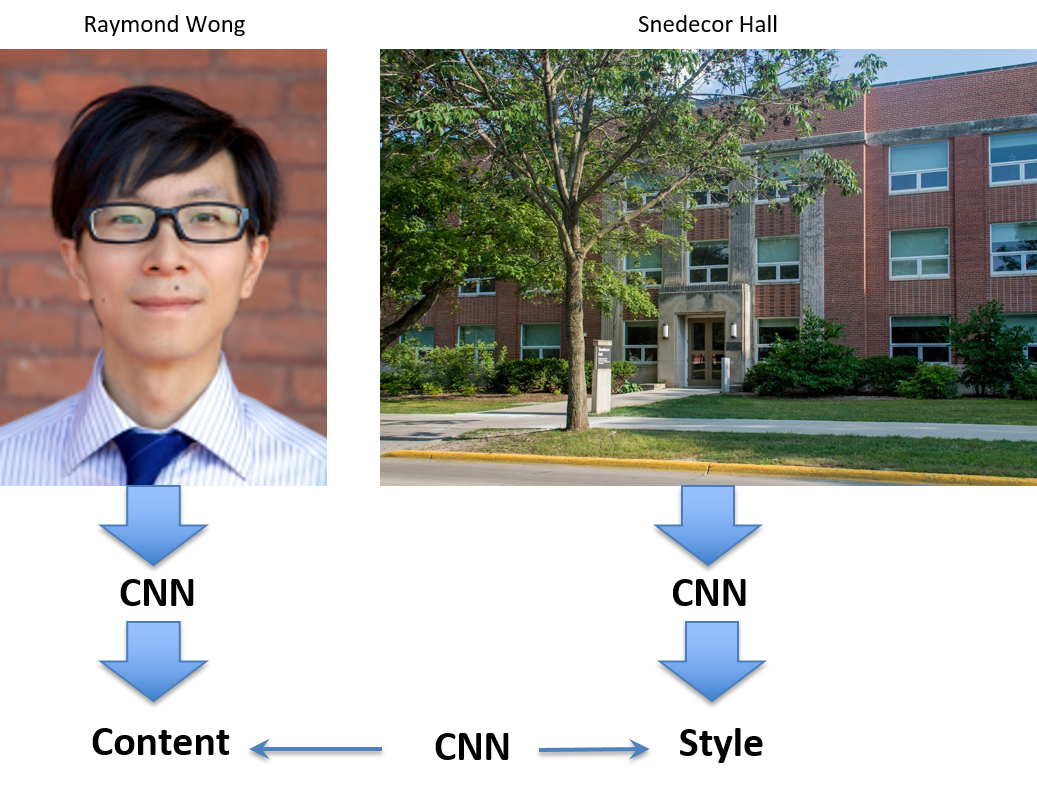
\includegraphics[width=0.8\linewidth]{Picture17}
	\end{figure}
\end{frame}
\begin{frame}
	\frametitle{Style Transfer}
\begin{center}
	Style Transfer, A.K.A. Deep Style
\end{center}
	\begin{figure}
		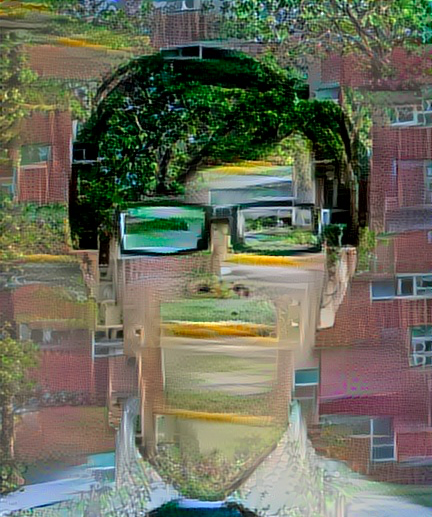
\includegraphics[width=0.5\linewidth]{style_transfer}
	\end{figure}
\end{frame}
%
%\begin{frame}
%	\frametitle{Style Transfer}
%		\begin{figure}
%			\hfill
%			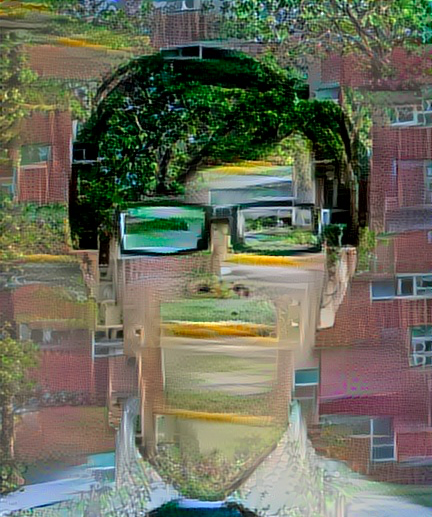
\includegraphics[width=0.5\linewidth]{style_transfer}
%			\hfill
%			Thank you!\\
%			
%			
%			Good luck with your finals!
%			\vspace{2in}
%			\hfill
%		\end{figure}
%\end{frame}
%
%
%
%
%\begin{frame}[fragile]{Lists}
%Items
%\begin{easylist}[itemize]
%@ Milk
%@ Eggs
%@ Potatos
%\end{easylist}
%
%Enumerations
%\begin{enumerate}
%\item First, \item Second and \item Last.
%\end{enumerate}
%
%Descriptions
%\begin{description}
%\item[PowerPoint] Meeh. \item[Beamer] Yeeeha.
%\end{description}
%\end{frame}
%
%\begin{frame}[fragile]{Tables}
%\begin{table}
%\caption{Largest cities in the world (source: Wikipedia)}
%\begin{tabular}{lr}
%\toprule
%City & Population\\
%\midrule
%Mexico City & 20,116,842\\
%Shanghai & 19,210,000\\
%Peking & 15,796,450\\
%Istanbul & 14,160,467\\
%\bottomrule
%\end{tabular}
%\end{table}
%\end{frame}
%
%\begin{frame}{Blocks}
%Three different block environments are pre-defined and may be styled with an
%optional background color.
%
%%   Color Box: Light Orange
%\setbeamercolor{boxsthlmLightOrange}{bg=white,fg=pblue}
%\begin{beamercolorbox}[wd=\linewidth,ht=10ex,dp=3ex]{boxsthlmLightOrange}
%\centering
%\texttt{Light Orange}\\
%\vspace{1em}
%\tiny{RGB:  255,215,210} \\
%\tiny{hex: \#ffd7d2}
%\end{beamercolorbox}
%\end{frame}
%
%\begin{frame}[fragile]{code}
%\begin{lstlisting}[language=JavaScript, caption=My Javascript Example]
%function someReducer(state = initialState, action) {
%  switch (action.type) {
%  case 'FOO':
%    return Object.assign({}, state, {
%      foo: action.payload.foo
%    });
%  default:
%    return state;
%  }
%}
%\end{lstlisting}
%\end{frame}

\end{document}
